\chapter{磁場中でのPMTの動作確認(担当:井口)}\label{PMT}

\section{動機}
磁場中のポジトロニウムの寿命測定実験(本実験)では,2インチPMT(光電子増倍管)とトリガー用の3/8インチPMTを磁場中で使用する.PMTは一般に磁場中ではゲインが低下してしまうため,あらかじめ磁場中でのPMTの動作を確認する必要がある.この章で述べる実験では,PMTを磁場中で使用した場合のゲインの変化を,$\gamma$線源のスペクトルを測定することで確認した.また鉄管でPMTを覆い同様の測定をおこなうことで磁場の遮蔽を試みた場合のゲインの変化を確認した.


\section{電磁石}
この実験では,本実験で使用する電磁石と同一の電磁石を用いる.はじめに電磁石に定格6.0 Aの電流を流し,ガウスメータを用いて,$z=0$ cmでの$z$方向の磁場の強さと$r$方向の関係を測定した.

\begin{figure}[h]
	\centering
	\includegraphics[width=15cm]{fig/iguchi/maggraph01.pdf}
	\caption{$z$方向磁場の$r$依存}
	\label{maggraph01}
\end{figure}

\newpage
\begin{itemize}
       \item 電磁石のN極からS極の方向を$z$方向とし,磁極間の中点を$z=0$ cmとする.
       \item 磁極の半径方向を$r$方向とし,磁極の中心を$r=0$ cmとする.
\end{itemize}


\begin{figure}[h]
	\centering
	\includegraphics[width=15cm]{fig/iguchi/magnetfigure.pdf}
	\caption{電磁石図}
	\label{magfigure}
\end{figure}

\begin{figure}[h]
	\centering
	\includegraphics[width=10cm]{fig/iguchi/magnetphoto.pdf}
	\caption{電磁石の写真}
	\label{magphoto}
\end{figure}




\section{2インチPMT}
使用したPMTは浜松ホトニクス製の光電子増倍管アッセンブリH6410で,ダイノード構造はラインフォーカス型である.
\begin{table}[h]
	\centering
	 \begin{tabular}{cccccccc}\hline
	型名& 管径 & 外径 & 長さ & 最大電圧 & 印加電圧 & ゲイン & ダイノード構造 \\ \hline \hline
	H6410 & 2 インチ & 60 mm & 200 mm & -2000 V & -1850 V & $3.0\times10{^{6}}$ &ラインフォーカス型 \\ \hline
	\end{tabular}
	  \caption{2インチPMTデータ表}
\end{table}

\begin{figure}[h]
  \begin{center}
    \begin{tabular}{c}
    %1
      \begin{minipage}[t]{0.5\hsize}    
        \begin{center}
          \includegraphics[width=6.5cm]{fig/iguchi/PMTphoto.jpg}
	\hspace{1cm}[1]2インチPMT H6410
     \end{center}
    \end{minipage}
    %2
      \begin{minipage}[t]{0.5\hsize}    
        \begin{center}
          \includegraphics[width=6.5cm]{fig/iguchi/PMTinner.pdf}
         \hspace{2cm}[2]ラインフォーカス型の内部構造
         \end{center}
        \end{minipage}
     
     \end{tabular}
     \label{PMT12}
    \end{center}
 \end{figure}

PMTを磁場中使用すると,光電子がPMT内部の磁場を進む間にローレンツ力を受けて軌道が曲がり,ダイノードに届かなくなりゲインが著しく低下する.


\section{測定方法と装置図}
2インチPMTの光電面にNaI(Tl)シンチレータを取り付け,$\ce{^{60}Co}$と光電面の距離を70 mmに固定し,磁場なしの場合と磁場ありのでゲインを測定した.また磁極の中心からPMTの光電面までの距離を$r$方向の距離とする.
 
\begin{figure}[h]
  \begin{center}
    \begin{tabular}{c}
    %1
      \begin{minipage}[h]{0.5\hsize}    
        \begin{center}
          \includegraphics[width=6.5cm]{fig/iguchi/2inchsokutei.pdf}
	\hspace{2cm}[1]測定装置
     \end{center}
    \end{minipage}
    %2
      \begin{minipage}[h]{0.5\hsize}    
        \begin{center}
          \includegraphics[width=6.5cm]{fig/iguchi/soutizu1.pdf}
         \hspace{2cm}[2]装置図
         \end{center}
        \end{minipage}
     
     \end{tabular}
     \label{souchi}
    \end{center}
 \end{figure}

\begin{figure}[h]
	\centering
	\includegraphics[width=5cm]{fig/iguchi/NaIscinti.jpg}
	\caption{NaI(Tl)シンチレータ}
	\label{NaIscinti}
\end{figure}

\begin{table}[h]
	\centering
	 \begin{tabular}{lcc}\hline
	種類& 直径 & 長さ \\ \hline \hline
	NaI(Tl)シンチレータ & 57 mm & 58 mm \\ \hline
	\end{tabular}
	  \caption{NaI(Tl)シンチレータデータ表}
\end{table}     
 
\subsection{2インチPMTの測定結果}

\begin{figure}[h]
	\centering
	\includegraphics[angle=-90,width=10cm]{fig/iguchi/121550on.pdf}
	\caption{$r=50$ cmのヒストグラム}
	\label{hist50}
\end{figure}

\begin{figure}[h]
	\centering
	\includegraphics[angle=-90,width=10cm]{fig/iguchi/121635on.pdf}
	\caption{$r=35$ cmのヒストグラム}
	\label{hist35}
\end{figure}

   
縦軸にPMTのゲイン,横軸にr方向の距離をとる.縦軸は磁場なしの場合のゲインで規格化した.磁場なしと$r=50,45$ cmのときは$\ce{^{60}Co}$の2つのピーク(1.17 MeV,1.33 MeV)が見える.$r=35$ cm(1.22 mTesla)ではゲインが大幅に低下した.$r=25$ cm(4.82 mTesla)では信号が消失した.
スペクトルのピークはガウシアンと一次関数でフィットした.$\ce{^{60}Co}$の2つのピークの形は同じだと考えて,ノイズは一次関数で表せると考えた.


\begin{figure}[t]
	\centering
		\includegraphics[angle=-90,width=10cm]{fig/iguchi/plot2inchPMT.pdf}
	\caption{2インチPMTの磁場中のゲイン変化}
	\label{plot2inchoff}
\end{figure}

この結果からPMTは$r=35 cm$,つまり$z$方向磁場の強さが1.22 mTeslaで使用出来なくなる。

\section{測定方法と装置図(鉄管あり)}
先述と同様の実験を,PMTを鉄管に入れるという条件のみ変えてゲインを測定した.


\begin{figure}[t]
  \begin{center}
    \begin{tabular}{c}
    %1
      \begin{minipage}[h]{0.5\hsize}    
        \begin{center}
          \includegraphics[width=6.5cm]{fig/iguchi/PMTinFe.pdf}
	\hspace{3cm}[1]鉄管内部図
     \end{center}
    \end{minipage}
    %2
      \begin{minipage}[h]{0.5\hsize}    
        \begin{center}
          \includegraphics[width=6.5cm]{fig/iguchi/jibakyusyu.jpg}
         \hspace{3cm}[2]磁性体によって吸収される磁場
         \end{center}
        \end{minipage}
     
     \end{tabular}
    \end{center}
   \end{figure}
   

\begin{figure}[h]
	\centering
		\includegraphics[width=7cm]{fig/iguchi/2inchinFe.jpg}
	\caption{測定装置(鉄管あり)}
	\label{2inchinFe}
\end{figure}


\begin{table}[h]
	\centering
	 \begin{tabular}{cccc} \hline
		素材 & 外径 & 内径 & 長さ \\ \hline \hline
		軟鉄 & 76.3 mm & 62.3 mm & 270 mm \\ \hline
	\end{tabular}
	  \caption{鉄管データ表}
	  \label{ironpipedata}
\end{table}

磁力線が鉄管端から内部に入り込む可能性を考慮して,鉄管端とPMTの光電面との距離が70 mmになるように取り付けた.
PMTを鉄管に入れる理由は,磁力線は磁化しやすい物質に吸収されるため,強磁性体の鉄管内部の磁場を遮蔽するためである.



\subsection{2インチPMT測定結果(鉄管あり)}

\begin{figure}[h]
	\centering
		\includegraphics[angle=-90,width=10cm]{fig/iguchi/122350fe.pdf}
	\caption{$r=50$ cm(鉄管あり)のヒストグラム}
	\label{hist50fe}
\end{figure}
\begin{figure}[h]
	\centering
		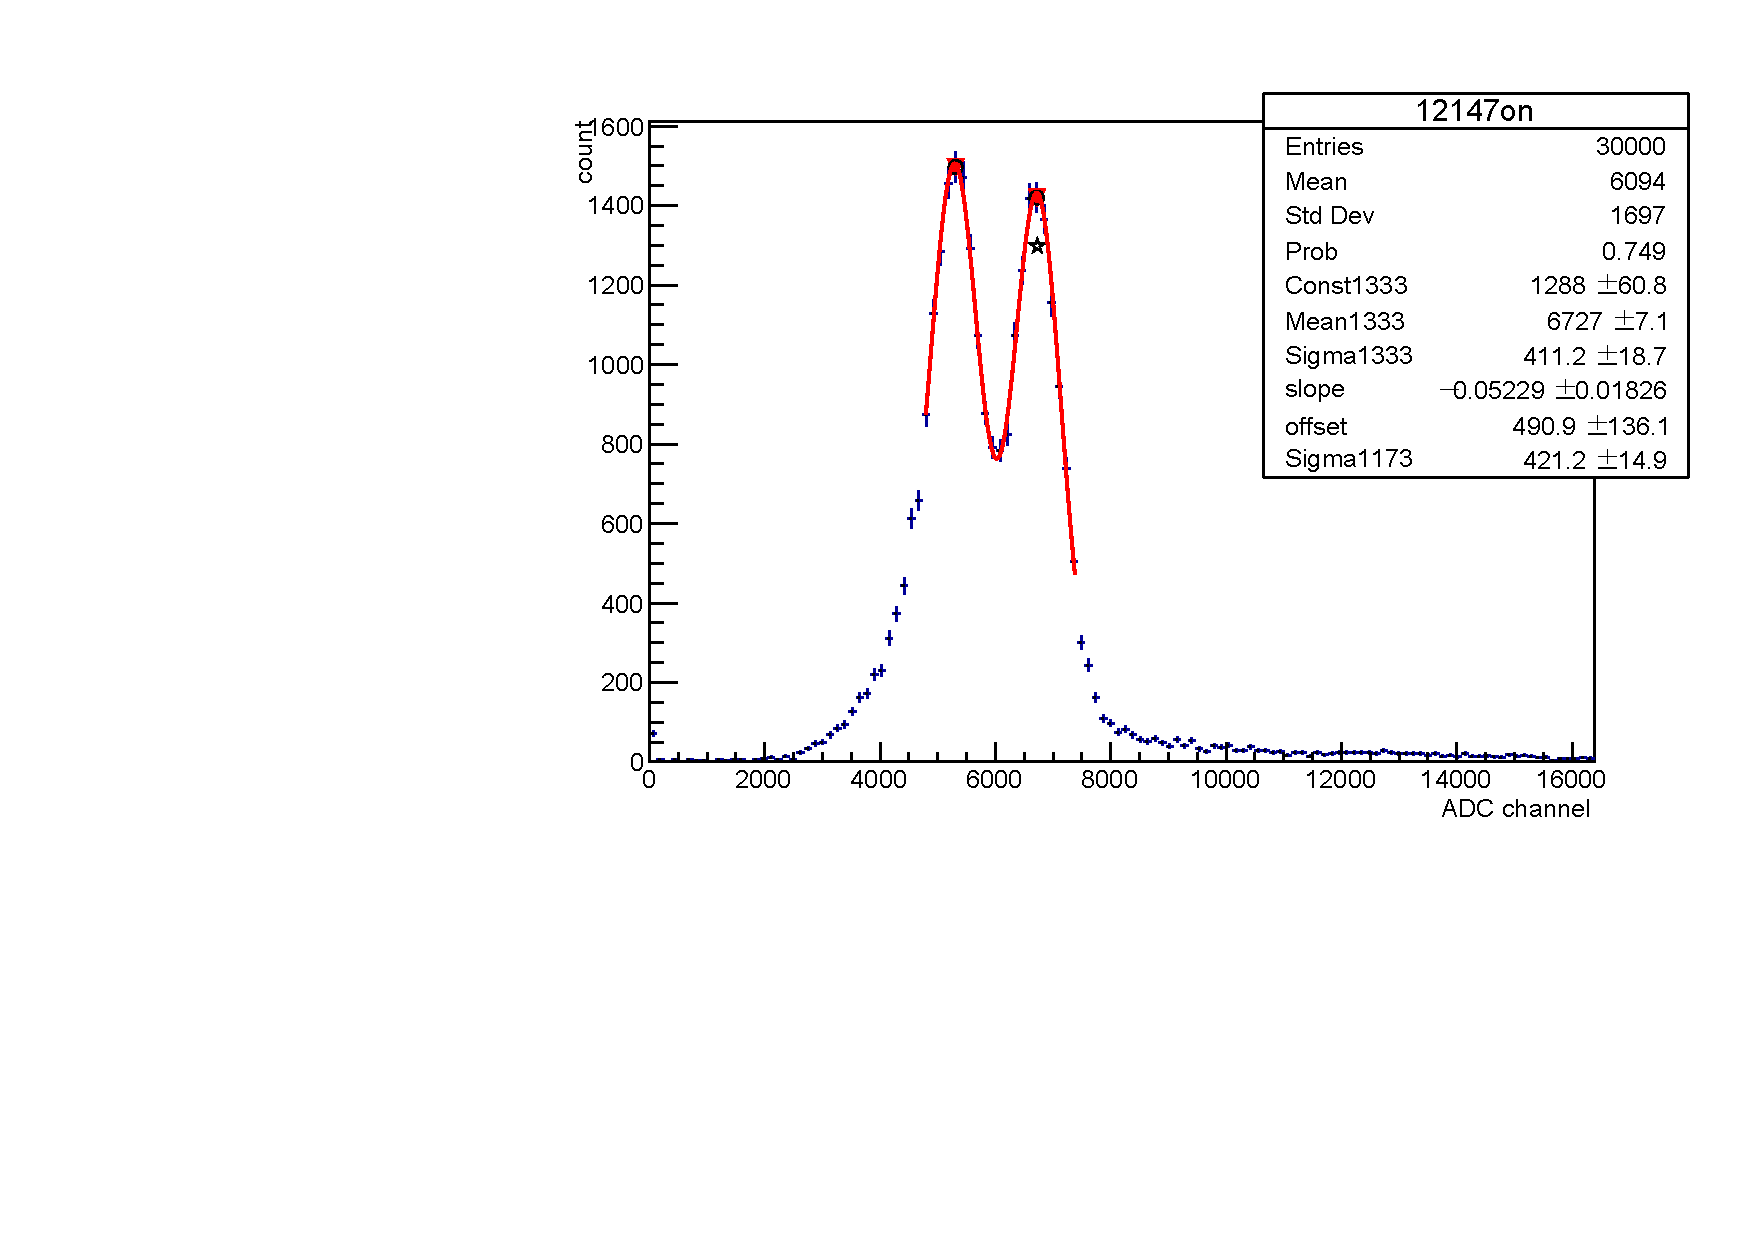
\includegraphics[angle=-90,width=10cm]{fig/iguchi/12147on.pdf}
	\caption{$r=7$ cm(鉄管あり)のヒストグラム}
	\label{hist7fe}
\end{figure}

\begin{figure}[h]
	\centering
		\includegraphics[angle=-90,width=10cm]{fig/iguchi/bigPMTfit.pdf}
	\caption{2インチPMTでの磁場中のゲイン変化(鉄管あり)}
	\label{bigPMTfit}
\end{figure}
鉄管なしの場合と同様の手法で規格化し,フィットした.$r=20$ cmまでゲインがほとんど低下せず,$r=20$ cm以下ではややゲインが低下するが,$r=7$ cmまで2つのピークを見ることができる.
本実験において2インチPMTは$r=12$ cmに設置する予定なので,鉄管に挿入し磁場を遮蔽することで,本実験でも使用可能である.

\newpage
\section{3/8インチPMTについて}
3/8インチPMTは,本実験ではトリガー用に使用されるため,2インチPMTより磁極に近い位置に設置される.
\begin{figure}[H]
	\centering
		\includegraphics[width=10cm]{fig/iguchi/miniPMT.jpg}
	\caption{3/8インチPMT H3164-10}
	\label{3/8inch}
\end{figure}
\begin{table}[h]
	\centering
	
	  \begin{tabular}{cccccccc} \hline
		型名& 管径 & 外径 & 長さ & 最大電圧 & 印加電圧 & ゲイン & ダイノード構造 \\ \hline \hline
		H3164-10 & 3/8 インチ & 10.5 ㎜ & 97 mm & -1500 V & -1400 V & $1.0\times10{^{6}}$ &ラインフォーカス型 \\ \hline
	\end{tabular}
	  \caption{3/8インチPMTデータ表}
\end{table}


\subsection{測定方法と装置図(3/8インチPMT)}

先述の実験と同様の方法で,$\ce{^{22}Na}$と3/8インチPMTの光電面との距離を100 mmで固定し,鉄管に入れた場合と入れない場合でゲインを測定した.
3/8インチPMTはダークカレントが多く線源のスペクトルが見えにくかったため,一つのNaIシンチレータに2つの3/8インチPMTを取り付け,それらの信号を同時計測することでダークカレントを落とした.


\begin{figure}[h]
  \begin{center}
    \begin{tabular}{c}
    %1
      \begin{minipage}[h]{0.4\hsize}    
        \begin{center}
          \includegraphics[width=6.5cm]{fig/iguchi/PPMT.jpg}
	\hspace{3cm}[1]3/8インチPMTのコインシデンス
     \end{center}
    \end{minipage}
    %2
      \begin{minipage}[h]{0.6\hsize}    
        \begin{center}
          \includegraphics[width=10cm]{fig/iguchi/miniset.pdf}
         \hspace{3cm}[2]3/8インチPMTの装置図
         \end{center}
        \end{minipage}
     
     \end{tabular}
    \end{center}
   \end{figure}
   

また鉄管は2インチPMTの実験で用いたものと同一のものを使用し,線源はスペクトルのピークの位置がわかりやすい$\ce{^{22}Na}$を使用した.


\subsection{3/8インチPMTの測定結果}

\begin{figure}[h]
	\centering
		\includegraphics[angle=-90,width=10cm]{fig/iguchi/minicoin22.pdf}
	\caption{$r=50$ cmのヒストグラム}(鉄管あり)
	\label{histminicoin22}
\end{figure}

\begin{figure}[h]
	\centering
		\includegraphics[angle=-90,width=10cm]{fig/iguchi/minicoin21.pdf}
	\caption{$r=6$ cmのヒストグラム(鉄管あり)}
	\label{histminicoin21}
\end{figure}

\begin{figure}[h]
	\centering
		\includegraphics[angle=-90,width=10cm]{fig/iguchi/minicoout22.pdf}
	\caption{$r=22$ cmのヒストグラム(鉄管なし)}
	\label{histminicoout22}
\end{figure}

\begin{figure}[h]
	\centering
		\includegraphics[angle=-90,width=10cm]{fig/iguchi/miniPMTgainG.pdf}
	\caption{3/8インチPMTの磁場中でのゲイン変化}
	\label{miniPMTgainG}
\end{figure}

先述の実験と同様に,横軸にr方向の距離,縦軸にゲインをとった.縦軸は磁場なしで測定したときのゲインで規格化した.また1.275MeVのピークはガウシアン+二次関数でフィットした.鉄管に入れない場合,$r=30$ cm(2.36 mTesla)まではゲインが低下しないが,$r=25$ cm(4.82 mTesla)付近からゲインが低下し,$r=22$ cm(10 mTesla以下)でゲインが低下しピークが見えなくなった.
鉄管に入れた場合,$r=6$ cmまでゲインが低下せず,スペクトルのピークがはっきり見える.


\section{3/8インチPMTの測定結果と磁場シミュレーション}
測定結果から3/8インチPMTはコインシデンスを取り,鉄管に入れることで$r=6$ cmまで使用できることがわかった.
しかし,本実験では3/8インチPMTは,外径21.7 mm,内径16.1 mmの鉄管に挿入し,3/8インチPMTを$r=2$ cmに設置する.(鉄管の端とPMT光電面の距離は5 mm)
\begin{figure}[H]
	\centering
		\includegraphics[width=10cm]{fig/iguchi/honjikken.pdf}
	\caption{本実験でのセットアップ}
	\label{honjikken}
\end{figure}
本実験をおこなう前に,上の条件でも3/8インチPMTが使用出来るかを確認するために,磁場シミュレーションソフト(Femtet)を使用した.
電磁石の磁場をFemtetで再現し,本実験で3/8インチPMTを使用する条件も再現し,鉄管内部の磁場をシミュレーションした.

\section{磁場シミュレーション結果}
\begin{figure}[h]
	\centering
		\includegraphics[width=16cm]{fig/iguchi/magnetgraph2.pdf}
	\caption{femtetで再現した磁場と実測定した磁場}
	\label{magnetgraph2}
\end{figure}

グラフから確認できるように,femtetで再現したz方向磁場と実際の測定結果を比較すると,ほとんど一致していることからfemtetの磁場シュミレーションは妥当であることがわかる.
\begin{figure}[h]
	\centering
		\includegraphics[width=20cm]{fig/iguchi/maggraphinFe.pdf}
	\caption{femtetで再現した磁場(鉄管あり)}
	\label{maggraphinFe}
\end{figure}
鉄管内部のz方向磁場のシミュレーション結果から,本実験で3/8インチPMTの光電面が設置される$r=2$ cmでの磁場の強さは1.5 mTeslaである.この結果と3/8インチPMTが使用可能であった$r=30$ cmでの磁場の強さ2.36 mTeslaを比較すると,シミュレーションの方が磁場が弱い.よって本実験でも使用可能であると結論付けられる.

\section{まとめ}




